% --------------------------------------------------------------
% This is all preamble stuff that you don't have to worry about.
% Head down to where it says "Start here"
% --------------------------------------------------------------
 
\documentclass[11pt]{article}

\usepackage{geometry} % Required for adjusting page dimensions

\geometry{
	top=1cm, % Top margin
	bottom=1.5cm, % Bottom margin
	left=3cm, % Left margin
	right=3cm, % Right margin
	includehead, % Include space for a header
	includefoot, % Include space for a footer
}


\usepackage[T1]{fontenc} % Output font encoding for international characters
\usepackage[utf8]{inputenc} % Required for inputting international characters

\usepackage{XCharter} % Use the XCharter font

\renewcommand{\thesubsection}{\thesection.\alph{subsection}}
\usepackage{todonotes}
\usepackage[margin=2cm]{geometry} 
\usepackage[backend=bibtex]{biblatex}
\addbibresource{ref.bib}
\usepackage[]{quoting}
\usepackage{listings}[language=C]
\usepackage{xcolor}
\usepackage{float}



\definecolor{codegreen}{rgb}{0,0.6,0}
\definecolor{codegray}{rgb}{0.5,0.5,0.5}
\definecolor{codered}{rgb}{0.64, 0.03, 0.22}
\definecolor{backcolour}{rgb}{0.9,0.9,0.9}

\lstdefinestyle{mystyle}{
    backgroundcolor=\color{backcolour},   
    commentstyle=\color{codered},
    keywordstyle=\color{magenta},
    numerstyle=\tiny\color{codegray},
    stringstyle=\color{codered},
    basicstyle=\ttfamily\footnotesize,
    breakatwhitespace=false,         
    breaklines=true,                 
    captionpos=b,                    
    keepspaces=true,                 
    numbers=left,                    
    numbersep=5pt,                  
    showspaces=false,                
    showstringspaces=false,
    showtabs=false,                  
    tabsize=2
}

\lstset{style=mystyle}

\usepackage{amsmath,amsthm,amssymb}
\usepackage[english]{babel} %Castellanización
\usepackage[T1]{fontenc} %escribe lo del teclado
\usepackage[utf8]{inputenc} %Reconoce algunos símbolos
\usepackage{lmodern} %optimiza algunas fuentes
\usepackage{graphicx}
\graphicspath{ {images/} }
\usepackage{hyperref} % Uso de links
 \hypersetup{
  colorlinks=true,
  linkcolor=blue!50!red
}

\begin{document}
 
% --------------------------------------------------------------
%                         Start here
% --------------------------------------------------------------
 
\title{MiniTwit Report \\
DevOps \\
BSDSESM1KU \\
(Data Science)}

\author{Anders Stendevald (andst@itu.dk) \\ 
Anna Reisz, (reis@itu.dk) \\ 
Edi Begovic (edbe@itu.dk) \\ 
Gergo Koncz (geko@itu.dk) \\ 
Høgni Jacobsen (hoja@itu.dk)\\
}

\maketitle
\clearpage
\section{Introduction}
MiniTwit is a Twitter clone originally written by ITU researchers. For some time, the web application has been neglected, with no maintenance being done. This changed in 2021. In the name of DevOps a handful of students decided to update it. 
\\\\
The following three sections will be covered: the System's Perspective (choices for the technology used in the project), Process' perspective (the way the team worked together and the how the decisions were made) and the Lessons Learned Perspective (our reflections on the project and the elements that we would have done differently).

\section{System's Perspective}
This section will cover the technical details of our system. We will discuss the considerations when creating maintainable software and explain the MiniTwit application and some of the most prominent technologies used in the project. Namely, Docker, Django, the CI/CD (Continuous integration and continuous delivery) chain, and our static Code Analysis.

\subsection{Creating maintainable software}
In a DevOps mindset, code should never be static and should always be up to date. One cannot be the only maintainer of an entire software stack. Therefore one should always strive to create software that can be forwarded to a new team without worry. This includes automation and giving an insight into how a piece of software should work (documentation). The target platform and dependencies should also be documented. It also means adopting a high standard of testing. Ultimately, a piece of software is only considered functioning when the code runs, the tests pass, and the documentation is clear. This is especially important in DevOps.
\\\\
The use of DockerFiles was especially important for this project (testing and deployments) as build steps are automated. This comes almost entirely for free, which makes it even more valuable to adopt Docker. 

%\subsection{What we need to do}
%A description and illustration of the:
% \begin{itemize}
%     \item Design of your ITU-MiniTwit systems
%     \item Architecture of your ITU-MiniTwit systems
%     \item All dependencies of your ITU-MiniTwit systems on all levels of abstraction and development stages.
%     \item That is, list and briefly describe all technologies and tools you applied and depend on.
%     \item Important interactions of subsystems
%     \item Finally, describe the current state of your systems, for example using results of static analysis and quality assessment systems.
%     \item Double check that for all the weekly tasks (those in the end of the lecture notes) you include the corresponding information.

% \end{itemize}
\subsection{Application / architecture overview}
% \begin{itemize}
%     \item Design of your ITU-MiniTwit systems
%     \item Architecture of your ITU-MiniTwit systems
%     \item All dependencies of your ITU-MiniTwit systems on all levels of
% \end{itemize}

At the core of our application, there are two Django applications interfacing with a single source-of-truth, a Postgres relational database. One of the Django applications is the web front-end for regular users, the other an API that provides access for developers. The rest of the architecture surrounding the core is to enable the maintenance, development, and evolution of the project in line with the DevOps mindset. Docker, Docker-compose, and Docker Swarm were utilized for virtualization and orchestration, Prometheus and Grafana for monitoring, and the ELK stack for logging. In figure \ref{fig:structure} there is a high-level overview of the architecture of our system.
\begin{figure}[h!]
    \centering
    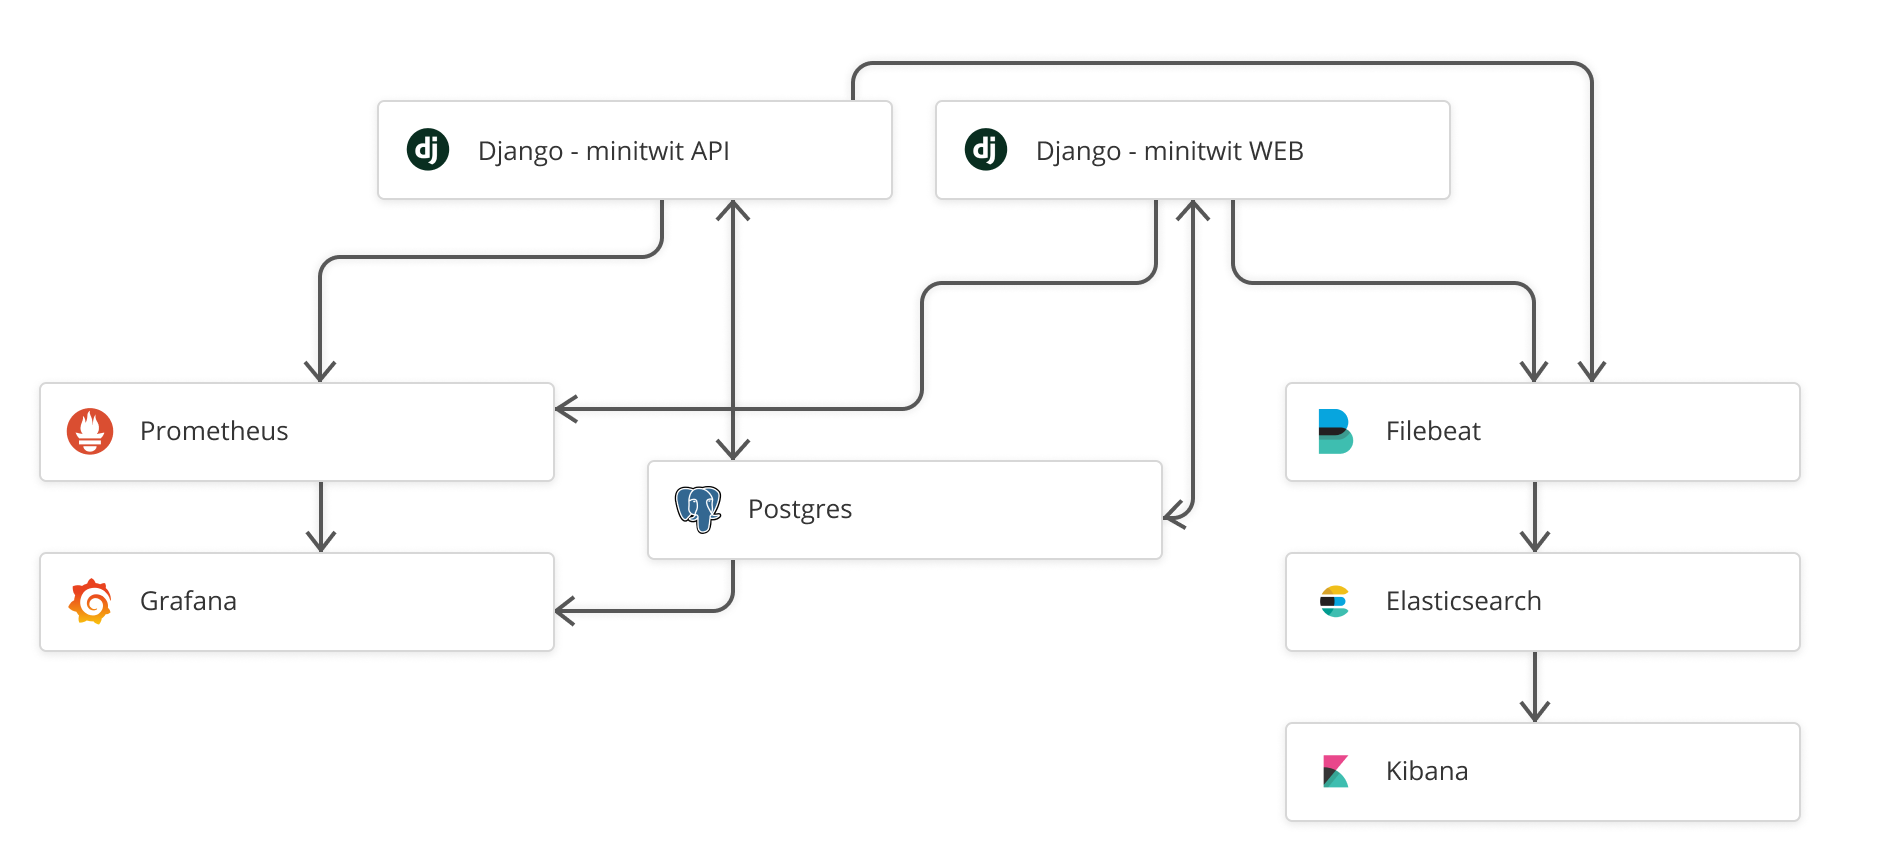
\includegraphics[width=16cm]{figures/structure.png}
    \caption{Application / Architecture overview. The components of the system and their connections. }
    \label{fig:structure}
\end{figure}
\ \\ \\ \\
\subsection{Virtualisation}
It was essential for the project to utilize virtualization. Not only would it make the application portable, but it also allows it to run on any platform. Below we will discuss why we chose Docker for virtualization instead of other technologies such as Vagrant. 

\subsubsection{Docker}
At the core of Docker is the Open Container Initiative\footnote{\url{https://opencontainers.org/}}. This means that Docker images adhere to specifications determined by domain experts, and thus running an application with Docker is not only cross-compatible today but also tomorrow.
\\\\
We decided to have all parts of the project in their own containers and images. The advantage of this was reduced development overhead and added security. The containers run without elevated user rights as the networking between containers is locked down. All of this was orchestrated with Docker compose, making the DockerFiles.   
\ \\

% \subsubsection{Not Vagrant}
The other option for a virtualization stack was Vagrant. We opted not to go for this because our application consisted of many small sub-components. Had we had a more complicated setup, with many connections between sub-components, Vagrant would have been easier. It also would have made it easier to deploy code to a new server. The overhead of developing on a Hypervisor would have made things complicated. For us, development in Docker was easier. 
\ \\ \\

\subsection{Core Technology stack}

\subsubsection{Django}
\href{https://www.Djangoproject.com/}{Django} is a Python library for web development. We chose this as our team had experience with Python, and Django is the "de facto" tool for full-stack Python web development. Django integrates well with the underlying database system and has multiple related tools that facilitate an ecosystem around web-based applications. 

Both our web and API interface is built on Django. The API orchestrates interactions with the database such as initial creation of tables, but both web and the API interact with the database directly during production.

\subsubsection{Postgres}
\href{https://www.postgresql.org/}{PostgreSQL} is one of the most prevalent relational database systems. It is open source and is nicely integrated with Django. Therefore it was the straightforward choice to store relational data. Postgres is also faster and scalable than SQLite, the original database system.


\subsection{CI-CD pipeline}
We decided to use GitHub actions to orchestrate continuous integration and development. We have found that this technology works inherently well with development using GitHub, generally speeding up development. GitHub enforced a DevOps-thinking that proved helpful when we needed to integrate more technologies on top of our existing stack. For example, we could use a marketplace action for pushing images to Docker Hub, which saved us development time.

\ \\
\noindent
We have implemented two pipelines. One functions as quality assurance (QA). Every time a fix/feature branch is merged into the development branch, we run some test scripts and perform linting. This script also deploys our project to a development environment. This being set up as a clone of the production environment, such that the system can be tested without the risk of failure or downtime on the production server.

\ \\
\noindent
The second action is used for deployment. In essence, it works the same way but is only triggered when we push code to the main branch, and it deploys our code to the production server. This step also includes creating a new release.

\ \\
\noindent
In figure \ref{fig:cicd_overview} we can see an overview of the CI/CD pipeline.

\begin{figure}[]
    \centering
    \makebox[\textwidth][c]{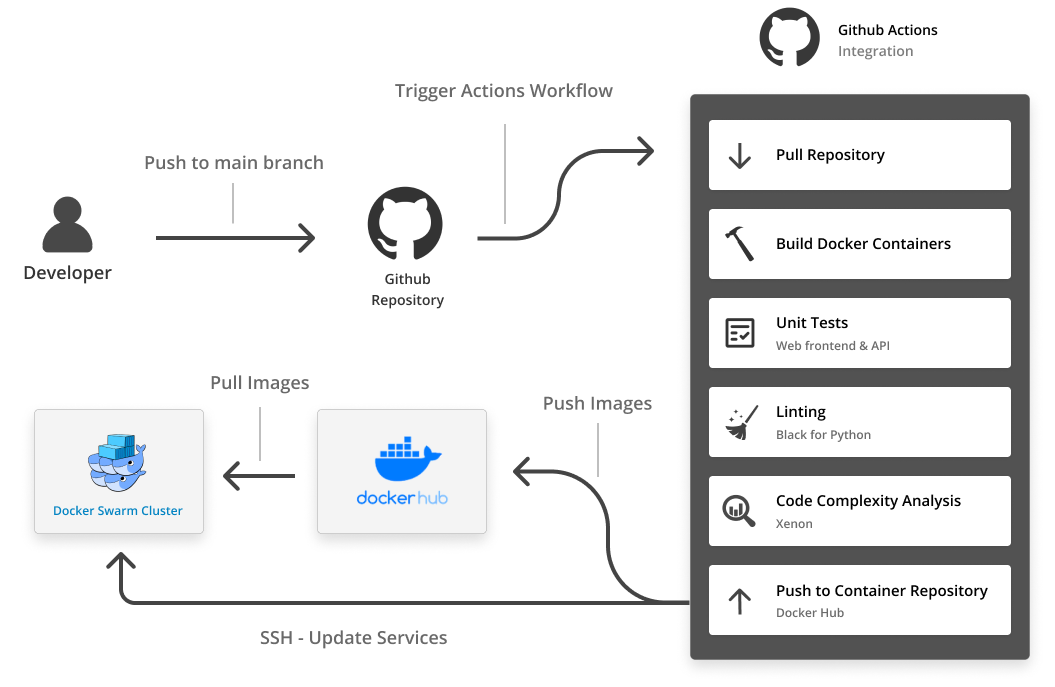
\includegraphics[width=1.0\textwidth]{figures/cicd_workflow.png}}
    \caption{CI/CD overview}
    \label{fig:cicd_overview}
\end{figure}

\ \\ \\ \\ \\ \\ \\ \\

\subsection{Linting}
For linting we used \href{https://github.com/psf/black}{Black} for Python, helping us to keep coding styles concise. Consistent code is easier to refactor, automate, test, and read.

\subsection{Static Code Analysis}
We are using \href{https://xenon.readthedocs.io/en/stable/}{Xenon} for static code analysis. Xenon is a Python tool that can assess code complexity. It is based on Radon, a tool that makes metrics based on the code's 
\href{https://radon.readthedocs.io/en/latest/intro.html}{cyclomatic complexity}. 

Xenon labels code files from A-F (A being the best). Our code passed with a B grade in \textit{block complexity, average complexity, modules complexity} and a grade A in module complexity and average complexity.

\subsection{License}
After careful inspection of our dependencies' licenses, we have decided to use the GPL3 license. This is mostly because one of our dependencies (psycopg2-binary) uses the same license which doesn't allow us to use to use a more open license such as MIT.

\subsection{Deployment}
As we were already using Docker containers, and as an extension, Docker compose, we chose to use Docker Swarm for orchestrating our services, as additional configuration is minimal. 
While Docker Swarm is great for horizontal scaling of state-less services (through the addition of multiple nodes), having multiple instances of databases to persist data can be troubling as race conditions can easily occur. 
\noindent
We therefore used DigitalOcean Droplets (acting as physical machines) for hosting our worker/manager nodes for the Swarm as well as a managed relational database running Postgres.

\section{Process' perspective}
The following section will cover the process elements of DevOps. This means the processes used to automate elements of development and the way the team, GitHub, and communication were set up. When creating an optimal process, it is important to adopt the right policies and ideas. Policies and ideas that make the project easier to work with, maintain, and handover — both from the perspective of the Developer, but also the other stakeholders.

\subsection{Logging and monitoring of the application}
The addition of logging and monitoring is crucial for detecting and identifying the events occurring, and that has occurred in the system. When proper logging is implemented, it is easier to fix errors, as with logging we can keep a tab of a vast amount of events, and with the help of the ELK (Elasticsearch, Logstash, and Kibana) stack, all these events are transformed to be consumable. Logging also makes it possible to show a newcomer how the application is used. With monitoring we can zoom in on events in a more focused and business-minded way.
\\\\
To monitor the system, we use database queries (Inside Grafana) and \href{https://github.com/giampaolo/psutil}{psutil} to pull system stats and pass them to Prometheus. We chose to monitor both business and technology-related metrics. Below we cover the prominent technologies used in our logging and monitoring.

\subsubsection{Prometheus}
\href{https://Prometheus.io/}{Prometheus} is a monitoring tool, which records events and metrics in a time-series database. We use Django-Prometheus, a library that integrates well with Django-based web applications. This monitors our Django models (directly from the database), the health of the server (such as CPU load and memory usage), web traffic (such as http response codes) etc. We also use Prometheus\_client for monitoring additional metrics. However, so far this was not necessary. 

\subsubsection{Grafana}
\href{https://grafana.com/}{Grafana} is an analytics visualization platform that displays dashboards of metrics provided by a monitoring tool such as Prometheus. Our dashboard  can be seen in \ref{fig:dash}. It is divided into two sections: one for technical purposes and one for business purposes. The technical part includes uptime, CPU load, memory usage, and disk usage. This gives us an overview of whether maintenance is needed at a glance. The business part includes the number of users, number of posts, and number of followers. This allows us to get a better overview of our product's popularity and makes us better understand how our users use the service.
\begin{figure}[h!]
    \centering
    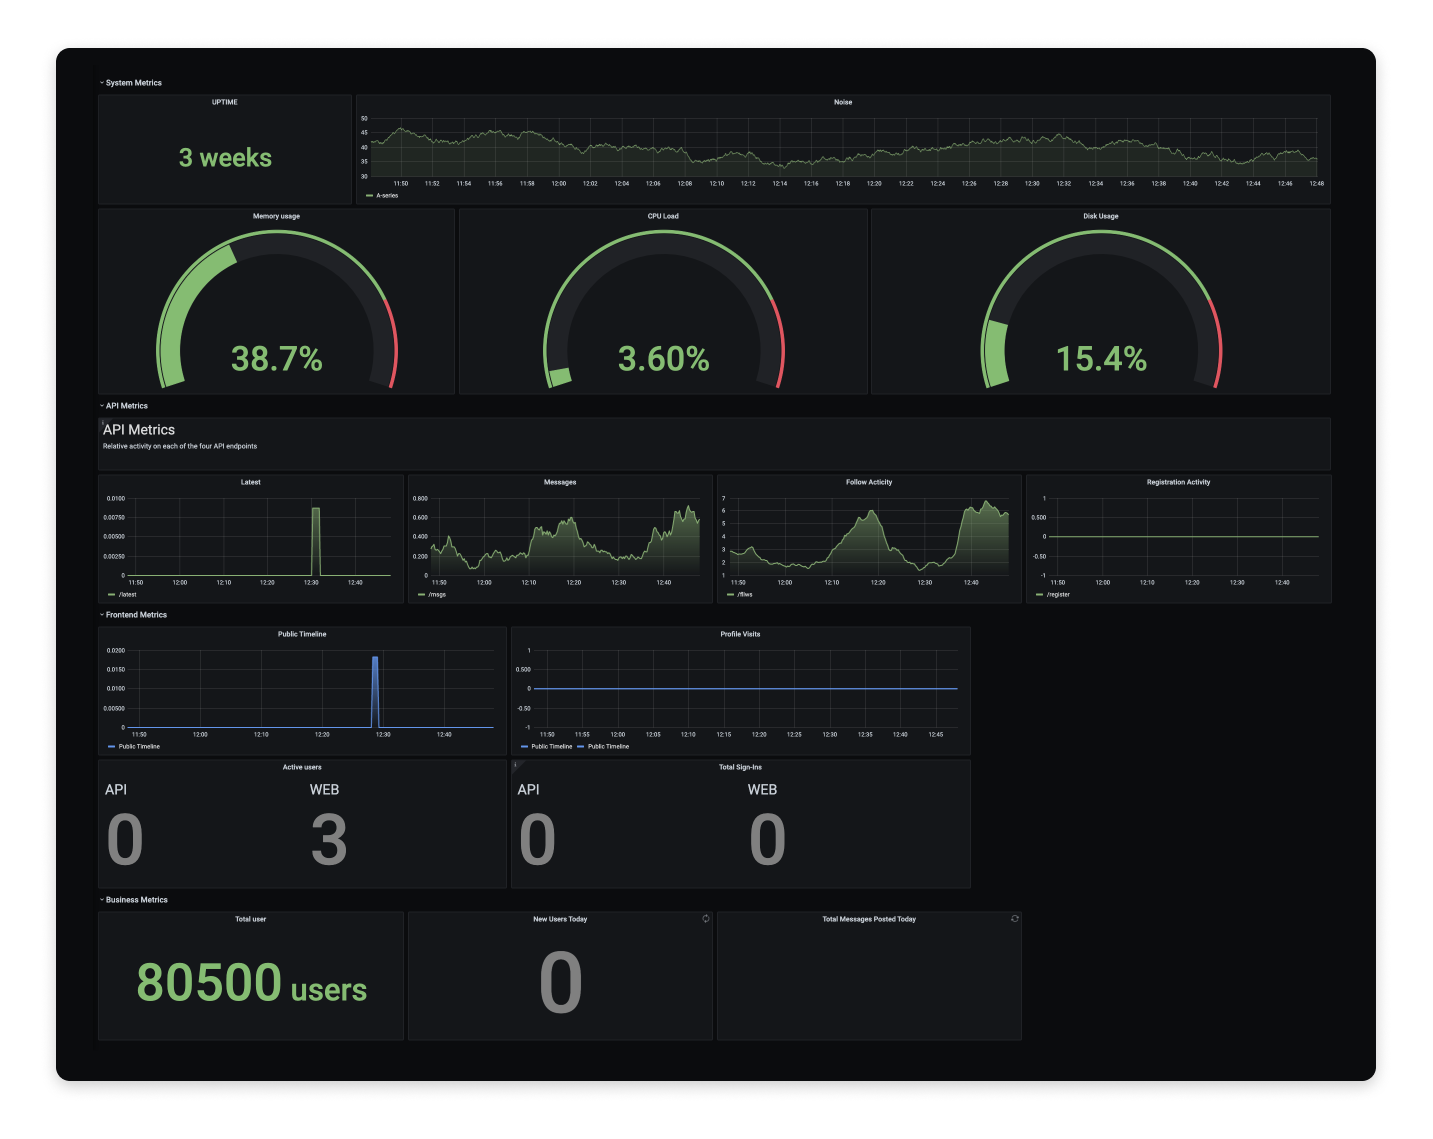
\includegraphics[width=16cm]{figures/dashboard.png}
    \caption{Grafana dashboard}
    \label{fig:dash}
\end{figure}

\subsubsection{Filebeat}
\href{https://www.elastic.co/beats/filebeat}{Filebeat} is a lightweight shipper for logs. Its function is to collect and centralize logs from given locations on the server and forward them to the specified target, ElasticSearch in our case. Using a Filebeat container was seamless in our setup. The configuration is about specifying where the log files are dropped and in what form Filebeat should forward them. 

\subsubsection{Elasticsearch}
\href{https://www.elastic.co/elasticsearch/}{ElasticSearch} is a multipurpose RESTful search and analytics engine with fast searching as the core feature. It is part of the ELK stack, and the software allows for several types of searches (structured, unstructured, geo, and metric). We have used an ElasticSearch to collect and structure the logs collected by Filebeat and allows for fast searching for the next tool in our logging pipeline.

\subsubsection{Kibana}
\href{https://www.elastic.co/kibana}{Kibana} is a flexible visualization tool that is the third element of the logging pipeline. Kibana transforms the logs structured by ElasticSearch into a more human-consumable format. Various visualizations can be utilized to make the logs more understandable and clearer.

\subsection{GitHub for collaboration}
As a development team, we mainly relied on having weekly meetings and discussing what product increments should be made. Afterwards we have been working on the new features in small teams or individually. To further improve on the organization of tasks, we made use of GitHub issues, allowing for easy integration with the concrete implementation through pull requests.
\\\\
We were keen on keeping a team of equal voices. However, if one of us had some previous experience with some technology to be implemented, then their voice and the arguments naturally carried more weight. Also, in case a person wanted to delve into some solutions more or experiment with alternative solutions for a given problem, it was encouraged. 
\\\\
We maintained two repositories, one for the CI part of the pipeline and for the CD. In the repository for CI we have contained the application code and the parts necessary for local development. Furthermore, GitHub actions for testing and building our Docker images, pushing them to the container registry. The deployment repository contained the configuration file needed for deploying to the test and the production server.
\\\\
Working with development in GitHub, we followed a strategy where the main branch was the base of releases (first, weekly, later automatic releases). We avoided committing directly to the main branch, instead merging development into main via a pull request. We usually agreed on these merges at a meeting as they had a significant impact on the overall project. All features and fixes were developed on feature branches which occasionally had sub-branches themselves when needed. Some of these sub-branches functioned as experiments and didn't lead anywhere. In contrast, others were merged back into the original feature branch, which was merged into the development branch as soon as the feature was complete. See Figure \ref{fig:branching}
\begin{figure}[h!]
    \centering
    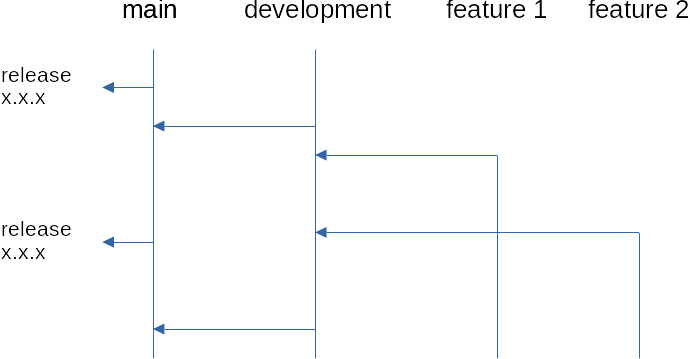
\includegraphics[width=12cm]{figures/branching.png}
    \caption{Branching strategy}
    \label{fig:branching}
\end{figure}
\subsection{Deployment and production CD}
Our GitHub action for deployment started with installing requirements, then testing our system both with scripts and static code analysis one last time, afterwards we built and pushed the images to Docker Hub. Finally, an update command is sent to the swarm, which pulls the images. This Docker compose file made sure that we started the database first, set up monitoring, then started our apps (API, then Web), and finally set up logging. The CD process ended with creating a new release.
\\

\subsection{Handling traffic}
There are three layers to handling incoming traffic to our system. 
Firstly, we use a DigitalOcean floating IP (Internet Protocol address) which is a flexible IP address that can be instantly mapped to any DigitalOcean service. A great advantage is the ability to experiment with different types of hardware without waiting 6-48 hours for the DNS (Domain Name System) to update the endpoint of our domain name. 
\ \\

\noindent
We use Docker Swarm to orchestrate the containers and allows us to seamlessly scale horizontally without having to manage "physical" machines or route traffic. Contrary to other distributed systems, the manager nodes don't only manage the incoming traffic. Instead, all nodes in the swarm are a part of a "routing mesh" which keeps track of which services run on all nodes. That way, incoming traffic to any node will automatically get routed to an instance of the service, even if it's not running on the actual node. Thus, the routing mesh also acts as a simple load balancer, spreading requests to the "least busy" instance of a service.
\ \\

Although the routing mesh provides load-balancing functionality, we further have an NGINX service running to route requests to the respective services. We went with NGINX due to its high configurability, e.g. allowing us to set up rules for sub domains. 

\begin{figure}[]
    \centering
    \makebox[\textwidth][c]{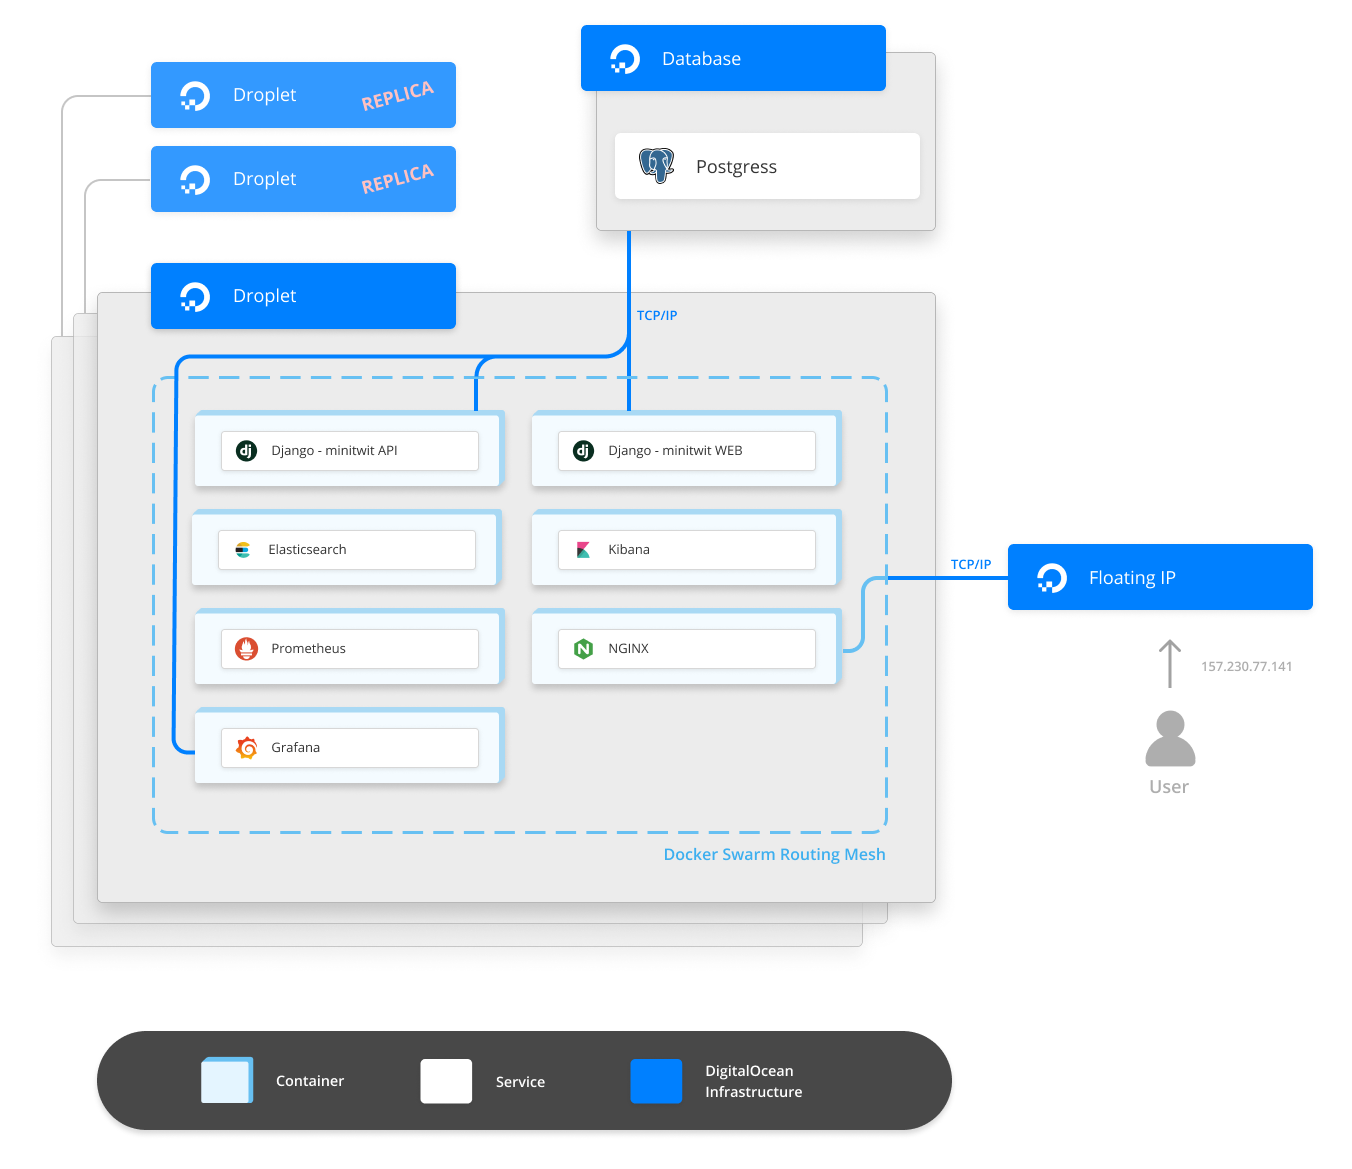
\includegraphics[width=1.2\textwidth]{figures/infrastructure.png}}
    \caption{Infrastructure overview}
    \label{fig:deployment_overview}
\end{figure}

\section{Lessons Learned Perspective}
This last section will conclude this DevOps project by highlighting the lessons learned in the project. In an iterative process, it is good to make mistakes as it is preferable from a learning perspective. This requires that mistakes are analyzed and discussed. Otherwise, a team might make the same mistake more than once. In this section, we highlight our venture into Kubernetes as a mistake and cover issues we had with Django (moving to), multi-App Django, and security.

\subsection{Kubernetes and its drawbacks}
During our final phases of development, we decided to adopt Kubernetes as our platform. We decided on the promise of rollover deployments, load balancing, centralized logging, and horizontal scaling. This move seemed straightforward, especially after we had containerized the entire stack of the application and supporting layers. Having infrastructure as code and deployments without having to rely on an SSH connection even for automated deployments.
\\\\
While every component worked fine internally and individually, we had problems configuring the incoming connections and putting at all together. You have to adhere to very strict and secure configurations with the network and load balancing when setting up the cluster. This is because Kubernetes is configured for security between layers and containers, with specific containers for handling and diverting connections. Therefore opening up a connection to the outside world is not possible with a one-line command, like you would do on a typical server.
\\\\
Even though every container has its own internal cluster IP, you cannot just use that IP to connect to a container long term. Cluster IPs are like workplaces with flowing seating. Today your API might have IP A, but tomorrow it might be IP Z. To solve this problem, you have labels on containers and other containers with selectors. This makes it possible for the selectors to figure out the cluster IPs of containers with the correct labels. 
\\\\
The takeaway is that you cannot hack your way to a small deployment of Kubernetes. In the end, the only way to configure Kubernetes is to have different layers with pods, deployments, services, load balancers, and namespaces. And this is without the complexity of Floating IPs and the setup that makes that work with load balancers. This is typically done by the cloud provider. And for our project, that would mean that we either needed to pay 10\$ a month for each External IP or that we need to configure an Ingress that needed to work with the Kubernetes setup. This ultimately was the final straw for us before we decided to stop our venture into Kubernetes.   

\subsection{Issues moving to Django}
The Old MiniTwit system was built on Python 2 and Flask. To migrate from Python 2 to 3 we used the Python module \href{https://docs.python.org/3/library/2to3.html}{2to3}. This did not work perfectly, and we had to change some code elements manually. Flask required some more work to migrate away from. To migrate from Flask we had to get an overview of the system in Flask and then we could then build the Django application up section by section. We ran into some issues due to us having two teams working on different parts of the refactoring. One working in the API the other on the web application. This issue was quickly fixed by consultation and a decision as to how to continue.

\subsection{Multi-App Django}

The system was supposed to work such that API is a back-end for Web and a standalone application interface. Unfortunately, achieving this with a Django-based infrastructure was not straightforward, and we ended with duplicates of configuration files and duplicates of system logic. We have solved the problem of inconsistent migrations in the database that the mirrored applications caused by appointing API as the orchestrator of database changes. This solution worked seamlessly when we started the simulation, but it can be troublesome to restart. In the future, we would like to investigate whether such a two-application two-interfaces one-database system can be solved with less duplication in a Django-based stack.


\subsection{Security}
Our current system has some major security weaknesses, as we didn't have time to come up with an elegant solution to address these issues. The biggest shortcoming of our system is the passwords are stored in plain text. This may be mitigated by using environment variables, which are stored as GitHub secrets. This comes with the added complexity of transferring the secrets to the target environment, which can potentially be done via GitHub actions. 
\\\\
However, we would have preferred to use the in-build functionality of handling sensitive variables via a dedicated security system such as the one that comes with the Kubernetes stack, as this would give us a better overview of these variables. We believe that as our system grows, it becomes increasingly important to address issues related to security and privacy. Therefore a dedicated security system would be a better choice for handling secrets. 
\\\\
Also, using SonarCloud we can see that the system is susceptible to Cross-Site Request Forgery.

\section{Conclusion}
In this project, we show one way of maintaining the systems of the MiniTwit application. Our emphasis on good quality assurance with automation shows the importance of DevOps. We show that the process is equally important as it serves to create the right environment for developing good software. We learned that the most high-tech technologies, like Kubernetes, might not be the right choice for any platform or team. That careful consideration are needed to determine the pros and cons of strategies.
\end{document}